
%mainfile: Networks.tex

\pagestyle{fancy} 
\lhead{Atelier Nueromodélisation, 2017}
\rhead{}
\rfoot{\thepage}
\cfoot{}
\lfoot{~\theauthor}
\renewcommand{\headrulewidth}{0.4pt}
\renewcommand{\footrulewidth}{0.4pt}


\title{Paper Implementation: Reproduce some basic results
of the article ``Generating Coherent Patterns of Activity from
Chaotic Neural Networks''\vspace{-0.5em}}
%\preauthor{} \postauthor{} 
\author{Hsieh Yu-Guan}
\date{\today}
\maketitle

\thispagestyle{fancy}

\setcounter{secnumdepth}{0}


\section{Summary}

In this report we'll be working on the article ``Generating Coherent
Patterns of Activity from Chaotic Neural Networks'' published by 
David Sussillo and L.F. Abbott in 2009. In the work of D. Sussillo and L.F.
Abbott, they were interested in neural networks that are capable of
generating complex activity patterns either spontaneously or in response to
different stimuli.

The network is meant to be chaotic before training, i.e.
its activity should be highly sensitive to initial conditions. This is
acheieved by the usage of strong recurrent synaptic connections inside it. 
The so-called FORCE learning algorithm is then employed to modify
synaptic weights either external to or within the network. 
After the training phase, the network will be able to produce a wide 
variety of complex output patterns and we can switch between different
outputs by controlling the input signal.

Now let's come back to this report itself. I only worked on a relatively 
small part of the article: the generation of periodic patterns in the 
absence inputs by using FORCE learning. Moreover, three distinct network
structures are considered in the article (this will be detailed later on), 
but only the first one, which is probably also the simpest, is implemented 
here.


\section{Introduction}

When we're performing some motor action, what is the source of the nerual
activity that initiates and carries out this behavior? In the paper of
D. Sussillo and L.F. Abbott, they examined the hypothesis that such actions 
may come from the reorgnaization of spontaneous neural activity, which then
leads us to another question: how can a such reorgnaization happen?

The objective is thus to find a possible synaptic weight modification rule
that allows the network activity to be reorgnaized into coherent patterns 
required to produce complex motor actions after training. However, comparing
with feedfoward architectures, the training of a recurrent network is
shown to be much more difficult due to several reasons.
First, feeding erroneous output back into a network during training may
prevent its activity from converging. Secondly, in a recurrent network
the credit assignement for output errors becomes quite a hard problem because
of the presence of recurrent weights. Finally, while using a network that
display chaotic activity prior to training can be beneficial, chaos
must be avoided during the learning phase.

FORCE learning solved these problems by keeping the errors always small
and forcing the synaptic modifications to be strong and rapid during traing.
This is quite different from classic learning algorithms which usually
reduce the errors little by little. Therefore, the goal of FORCE learning
is not significant error reduction, but rather reducing the amount of
modification needed to keep the errors small.

According to the article, the contribution of FORCE learning can be
viewed from two different angles. From a biological point of view, it can
be regarded as a model for learning-induced moficifation of biological
models. Or more simply, it can just be seen as a powerful algorithm that
is able to construct recurrent networks being able to generate complex
and controlable output patterns.


\section{Network Structures}

The network that was studied in the paper and will be study here is composed
of individual neurons characterized by their firing rates and
sparsely interconnected through excitatory and inhibiroty synapses of 
various strengths (when it comes to the biological reality, we may need to
seperate group of excitatory and inhibitory neurons, but when we're modeling
neural circuits, such details become less important). Initially, the
connectivity and synaptic strengths of the network are chosen randomly.

The next problem is the definition of the output of the networks. The
technical choice is to define it as a linear combination of neuronal
activities. Formally, if at time $t$, we assemble the firing rates of all
the neurons into a column vector $\mathbf{r}(t)$, and the weights 
connecting these neurons to the output is described by the column vector
$\mathbf{w}(t)$, then the network output is

\[z(t) = \mathbf{w}^{\top}\mathbf{r}(t).\]

Schematically, this output will be stored in a readout unit and its
value may be fed back into the network (it depends on the concrete
structure). Though thus far the network output is only a scalar, by using
several differents decoding vectors $\mathbf{w}$ we can easily define
a multidimensional readout. This is exactly what D. Sussillo and L.F.
Abbott did in their paper when they later asked the network to generate
multiple outputs; however this point will not covered by the report.

Now that we have defined $z$ as the output of the network, the goal
of the algorithm is to set $z = f$ for somme target function 
$f: t \mapsto f(t)$. Either $z$ is generated in the abscence of any input
or it may depend on inputs of the network in a specific way. In the scope
of this report, only the first case will be discussed.

Finally, as shown in \autoref{fig: network_structures}, three different 
network structures are proposed in the article. In the first structure
(\autoref{fig: network_structures}A)
the feedback to the generator network is provided directly from the readout
unit. During training, we modify only the decoding vector $\mathbf{w}$
and the internal recurrent synaptic strengths are left intact.
Such a network is simple but far from realistic: every neuron receives the
same feedback (though it may be weighted differently) and this feedback
itself originates from an abstract output that doesn't exist in real circuit.
To address this problem, two other structures more biologically plausible
are given. In the second structure (\autoref{fig: network_structures}B)
we use a separated feedback network to supply feedback and in the third one 
(\autoref{fig: network_structures}C) modifications on internal synaptic
strengths are allowed. Without giving more details here, I just mention 
that after proper adaptions, FORCE learning can be carried out on the
three structures and yield promising results indifferent to the
underlying network structure.

\begin{figure}[H]
  \centering
  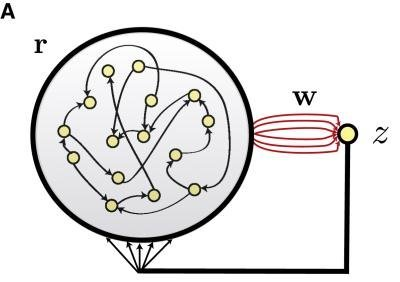
\includegraphics[width=0.32\textwidth, valign=t]{network_structure1}
  \hfill
  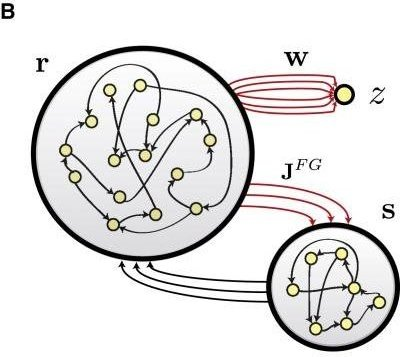
\includegraphics[width=0.32\textwidth, valign=t]{network_structure2}
  \hfill
  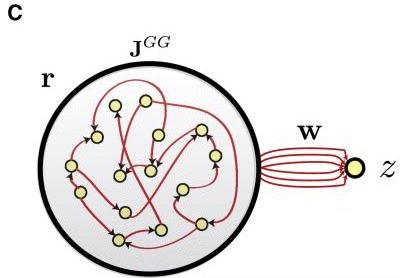
\includegraphics[width=0.32\textwidth, valign=t]{network_structure3}
  \caption{
    \textbf{Network Architectures (picture from the paper).}\\[0.1em]
    In all three cases, a linear readout unit derives an output $z$
    from the firing rates $\mathbf{r}$ of the recurrent generator network.
    Only connections shown in red are subject to modification.\\[0.1em]
    (A) The output of the readout unit is directly fed back to the
    generator network.\\[0.1em]
    (B) Feedback to the generator network is provided by a separated
    feedback network recurrently connected and whose inputs come from
    the generator network through synapses of strength $\mathbf{J}^{FG}$
    (red) that are also modified during training.\\[0.1em]
    (C) A simple recurrent network with no external feedback, but all
    synaptic strengths $\mathbf{J}^{GG}$ are subject to be modified by 
    the learning algorithm.
  }
  \label{fig: network_structures}
\end{figure}

Now let's put all the elements together and give a formal description of
the network that will be used in the framework of this report. First
we have a column vector $\mathbf{x}$ containing some abstract values of
each neuron (just for modeling convenience, or one may be able to find
some biological meaning for this vector that I ignore here). The firing
rates are computed by $\mathbf{r} = \tanh(\mathbf{x})$ (application of
the function term by term). The dynamic of the network is governed by
the equation

\[
  \tau \frac{d\mathbf{x}}{dt} = 
  -\mathbf{x} + g_{GG}\mathbf{J}^{GG}\mathbf{r}
  + g_{Gz} \mathbf{J}^{Gz} z,
\]

where $\tau$ is the caracteristic time, $\mathbf{J}^{GG}$ and 
$\mathbf{J}^{Gz}$ are respectively the matrix of internal synaptic 
weights and the vector of connection weights from the readout unit 
to the generator network (the feadback loop), and $z$ is the output
defined earlier. $g_{GG}$ is introduced to scale the strengths of 
the recurrent connections. When $g<1$ the network is inactive prior to
training; on the contrary if $g>1$ the network exhibits chaotic spontaneous
activity. $g_{Gz}$ plays a similar role with regard to the connections
from the readout unit to the main network.

We use moreover a sparseness parameter $\rho$ to impose sparsity on the 
network: each pairwise connection is set and held to 0 with probability 
$1 - \rho$. In the whole report, we'll choose $\tau=10$ ms, $g_{GG} = 1.5$,
$g_{Gz} = 1$, and the network contains $N=1000$ neurons unless otherwise 
stated. For initialization, nonzero elements of $\mathbf{J}^{GG}$ are drawn
independently from a Gaussian distribution with zero mean and variances
$1/(\rho N)$ while elements of $\mathbf{J}^{Gz}$ are drawn from a uniform
distribution between -1 and 1. We notice that feedback synapses are stronger
than internal ones in order to have an appreciable effect on the
network activity and this is necessary for suppressing the inherent
chaos of the network. Similarly, elements of $\mathbf{w}$ and 
$\mathbf{x}$ are respectively generated by Gaussian distributions with zero 
means and standard deviations $\sqrt{1/(\rho N)}$ or $\sigma_x = 0.5$.


\section{FORCE learning}

The term FORCE learning stands for first-order reduced and controlled error
learning. Training of recurrent networks is in general a hard problem as 
already mentioned in the introduction (even though here we modify only
the readout vector $\mathbf{w}$, the presence of the feedback loop makes
any effect of the modification difficult to predict). Since erroneous output
shouldn't be fed back to the network, the proposed algorithm must rapidly 
reduce the magnitude of the difference between the actual and desired output
to a small value, and then keep it small while searching for the proper
fixed readout vector that can generate the target function without further
modification of this vector.

The general schema of such an algorithm consists of updating $\mathbf{w}$
at times separated by an interval $\Delta t$ based on the readout error
at this moment which is defined by:

\[e_-(t) = \mathbf{w}^{\top}(t-\Delta t)\mathbf{r}(t) - f(t).\]

\noindent
The minus subscript signifies that this is the error prior to weight update 
at time $t$. The update of $\mathbf{w}(t-\Delta t)$ to $\mathbf{w}(t)$ should
allow us to decrease the error so that

\[e_+(t) = \mathbf{w}^{\top}(t)\mathbf{r}(t) - f(t)\]

\noindent
satisfies $|e_+(t)| < |e_-(t)|$. Since the end of the training takes place
only when the decoding vector $\mathbf{w}$ stabilizes and no longer changes,
this also requires $e_+(t)/e_-(t) \rightarrow 1$. 
Note that $\Delta t$ is the interval of time
between modifications of readout weights and doesn't necessarily equal to
the basic integration time step for the network simulation. In fact,
for the simulations carried out throughout this report, I take 
$\Delta t = 1$ ms whereas the basic integration time step is 0.1 ms.

Knowing all of this, it's still far from obvious to deduce the appropriate
modification rule that will work. In the paper, D. Sussillo and L.F. Abbott
express their favor to use the recursive least-squares (RLS) algorithm here.
I'll not dig into the mathematical details of this algorithm, but briefly
in our case it gives

\[\mathbf{w}(t) = \mathbf{w}(t-\Delta t)
                - e_-(t)\mathbf{P}(t)\mathbf{r}(t),\]

\noindent
where $\mathbf{P}(t)$ is an $N \times N$ matrix that is updated at the same
time as the weights according to the rule

\[\mathbf{P}(t) = \mathbf{P}(t-\Delta t) 
  - \frac{\mathbf{P}(t-\Delta t)\mathbf{r}(t)\mathbf{r}^{\top}(t)
    \mathbf{P}(t-\Delta t)}
    {1 + \mathbf{r}^{\top}\mathbf{P}(t-\Delta t)\mathbf{r}(t)}.\]

\noindent
We set the initial value for $\mathbf{P}$ to be 
$\mathbf{P}(0)=\mathbf{I}/\alpha$
where $\mathbf{I}$ is the identity matrix and $\alpha$ is a constant parameter
that needs to be chosen carefully
according to the target function being learnined. In this report I use
$\alpha = 1$ as suggested by the article. The modification rule can
then be viewed as a starndard delta-type rule, but instead of a scalar
quantity, multiple learning rates are specified by $\mathbf{P}$, which is
in reality a running estimate of the quantity 
$(\sum_t \mathbf{r}(t)\mathbf{r}^{\top}(t) + \alpha \mathbf{I})^{-1}$.
The use of $\mathbf{P}$ allows us to have a finer control over learning
because it adapts the learning rate to the magnitude of different principal
components of the network activity. However, concerning how it works and
why it works, it will no be explained here.

One can easily show that if we assume that $\mathbf{w}(0) = \mathbf{0}$
for simplicity, the error after the first weight update at time $\Delta t$
is

\[e_+(\Delta t) = - \frac{\alpha f(\Delta t)}
                {\alpha + \mathbf{r}^{\top}(\Delta t)\mathbf{r}(\Delta t)}\]

\noindent
which is small as long as $\alpha \ll N$ knowing that 
$\mathbf{r}^{\top}\mathbf{r}$ is of order $N$. Furthermore, every time
when the weights are updated, we have

\[e_+(t) = e_-(t)(1-\mathbf{r}^{\top}(t)\mathbf{P}(t)\mathbf{r}(t)).\]

\noindent
The quantity $\mathbf{r}^{\top}\mathbf{Pr}$ is always positive and
decreases to zero over the course of learning; this means the size of 
error is reduced by the weight update and as required 
$e_+(t)/e_-(t) \rightarrow 1$.


\section{FORCE Learning Examples}

In this section we'll apply the FORCE procedure on the network for different
target functions. The network is able to learn to generate a variety of
patterns after training. The first example presented here is a 
triangle wave of period 0.6 s (\autoref{fig: triangle}). 
The network activity is chaotic before training 
(\autoref{fig: triangle}A, blue lines), and 
during the training phase (\autoref{fig: triangle}B), 
as predicted the error is reduced dramatically after a first weight
update and the output of the network (red line)
matches target function throughout
the rest of training. The progression of learning can be observed through
the decrease of size of fluctuations of the readout vector
(orange trace). $\mathbf{w}$ 
fluctuates rapidly at the beginning of training to force the network
to produce the desired periodic pattern, but gradually it stabilizes and
find the static weights that are needed to generate the target function
without requiring modifications. 
After training (\autoref{fig: triangle}C), the network continues
to generate the desired pattern indefinitely without need of modifcation 
on decoding weights.

We also notice that the network activity chaotic prior to training 
becomes periodic in order to produce the periodic target function, and
it continues to be periodic after learning. The learning process is indeed
quite rapid here, only five cycles of the traingle wave is sufficient 
here (and in the paper the convergens takes place only after four cycles).
This time depends however a lot on the form of the target function.
For example, to learn the complicated periodic functions shown in
\autoref{fig: patterns}B, the network needs to be trained for a time
that corresponds to 10 to 20 cycles of this function ($\sim 30$ s).
And for the sine wave with extremely small period (\autoref{fig: patterns}D),
hundreds of cycles are even needed since the network converges only
after a few tens of seconds.

As a matter of fact, we show in \autoref{fig: patterns} that the network
is able to produce periodic functions of different complexity and form, 
even when the target function is corrupted by noise 
(\autoref{fig: patterns}E). Nonetheless, the article claims that in these
examples, training typically converges in $1000\tau$, that is, 10 s, while
in my simulations it takes much longer time. In most of the cases,
at least half a minute is required for the convergence to take place and 
sometimes even longer time is needed. For example, in 
\autoref{fig: patterns}D the network is trained for a minute 
(simulation time) but the generated sine wave is still not yet perfect.

According to the paper, with the parameters that are used here,
the network is able to generate sine wave with periods ranging from 60 ms
to 8 s after training. As just mentioned, though not perfect, I managed
to reproduce this result for a sine wave with period 60 ms. This is
however not the case for a sine wave with period 8 s 
(\autoref{fig: sin_8s}). We see that after one and half a minute of training
the network is still not able to produce the target funciton.
I don't know that if more time is needed for the training to converge 
since the function is of great period or my network is just not able to
learn to produce this function using the FORCE procedure.

In the paper, it is also shown that using FORCE learning the network is
capable of producing non-periodic functions as well, such as the dynamic 
variables of the three-dimensional chaotic Lorenz attractor (even though the
match lasts only for a finite amount of time). By modifying slightly 
the network structure and the training algorithm (adding a second readout
unit and feedback loop), it's also possible to produce a segment matching
a one-shot target function. However, due to the complexity of these two
experiments, they're not reproduced in my report.

Another point worth mentioning is that with the presence of feedback loop
and if the parameters are initialized as described above, the network is in
fact incapable of displaying spontaneous chaotic activity in my simulation.
Two possible scenarios are present, the whole system can converge
to some fixed point and become inactive (\autoref{fig: no_chaos}) or 
the network activity may become periodic (\autoref{fig: small_sin}A).
As a result, in \autoref{fig: triangle} I in fact set $g_{Gz}=0$
before training to exhibit the chaotic behavior. Since the initial value
of $\mathbf{x}$ doesn't seem to be important for FORCE learning, the fact
that the network doesn't demonstrate chaotic activity when there is 
feedback and when the parameters are initialized in the way described earlier
has no influence on the learning procedure that takes place later. 

A possible hypothesis is that strong feedback connection 
weights $\mathbf{J}^{Gz}$ may prevent the network from being chaotic
in any situations even when training is not taking place. This explication
can however be denied by \autoref{fig: small_sin}.
In this figure two things are shown: since strong feedbacks are
indespensable for suppressing the chaotic behavior of the network,
when the target function has a too small magnitude the activity
of the network neurons is chaotic during training and learning doesn't
converge to a successful solution. According to the paper, this problem
wouldn't occur with the networks shown in 
\autoref{fig: network_structures}B and 1C.
The second obeservation is more interesting, the network activity is in fact
not chaotic before training, but it becomes chaotic during learning and
remains chaotic even after learning. This suggests that even with the
presence of feedback loop the network can be spontaneously chaotic.
One possible reason is that after learning the output $z$ becomes
smaller in magnitude (this can be seen in the figure) and the feedback
into the network is now too small to suppress the chaos. This explanation
is still far from satisfying since the change of $|z|$ is not always 
significant but by traing the network with a target function with small
magnitude we are always able to exhibit chaotic activity at the end.
I really have difficulty in finding a good reason to explain this.

\begin{figure}[H]
  \centering
  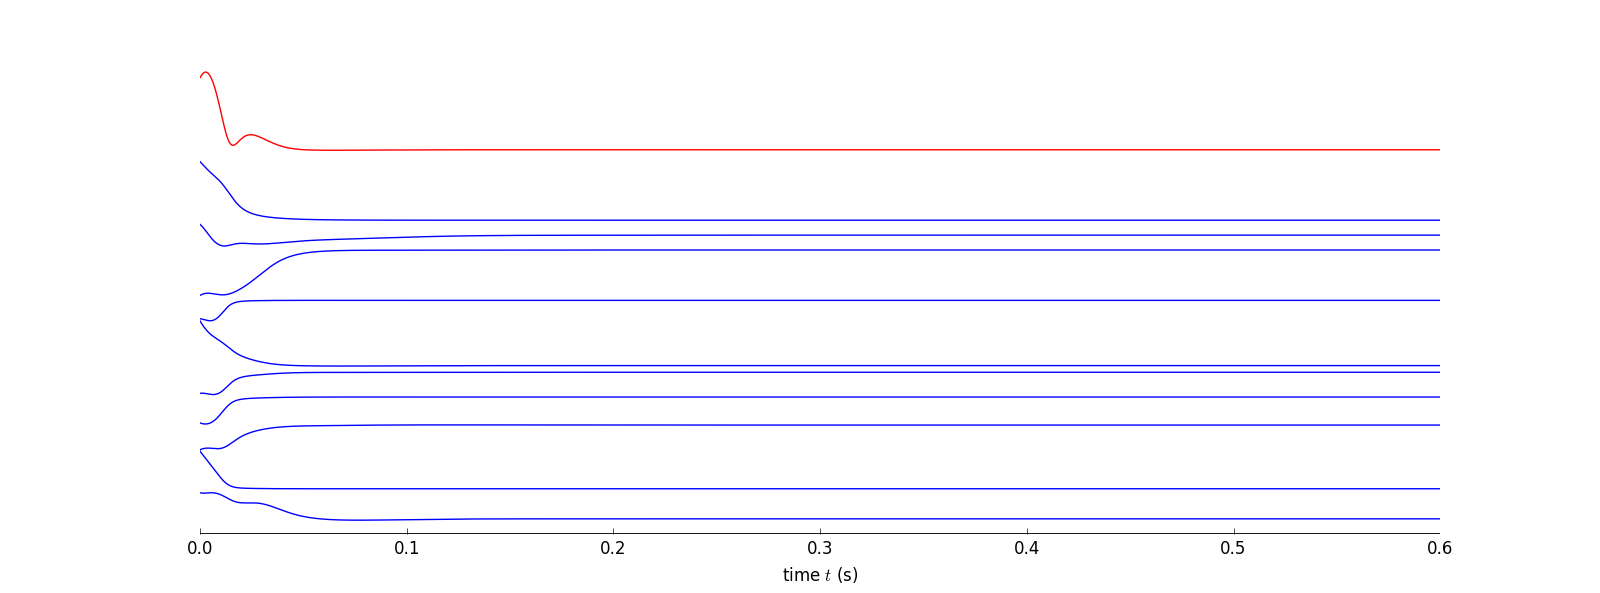
\includegraphics[width=\textwidth]{no_chaos}
  \caption{
    \textbf{Network Spontaneous Activity with the Presence of Feedback Loop.}
    \\[0.1em]
    When the feedback loop is present (so $g_{Gz}=1$) and the initialization
    is carried out as decribed in the text, the network doesn't exhibit 
    chaotic activity prior to training. In this figure the system converges to
    a fixed point and becomes inactive.
  }
  \label{fig: no_chaos}
\end{figure}

\newpage

\vspace*{-1em}
\begin{figure}[H]
  \centering
  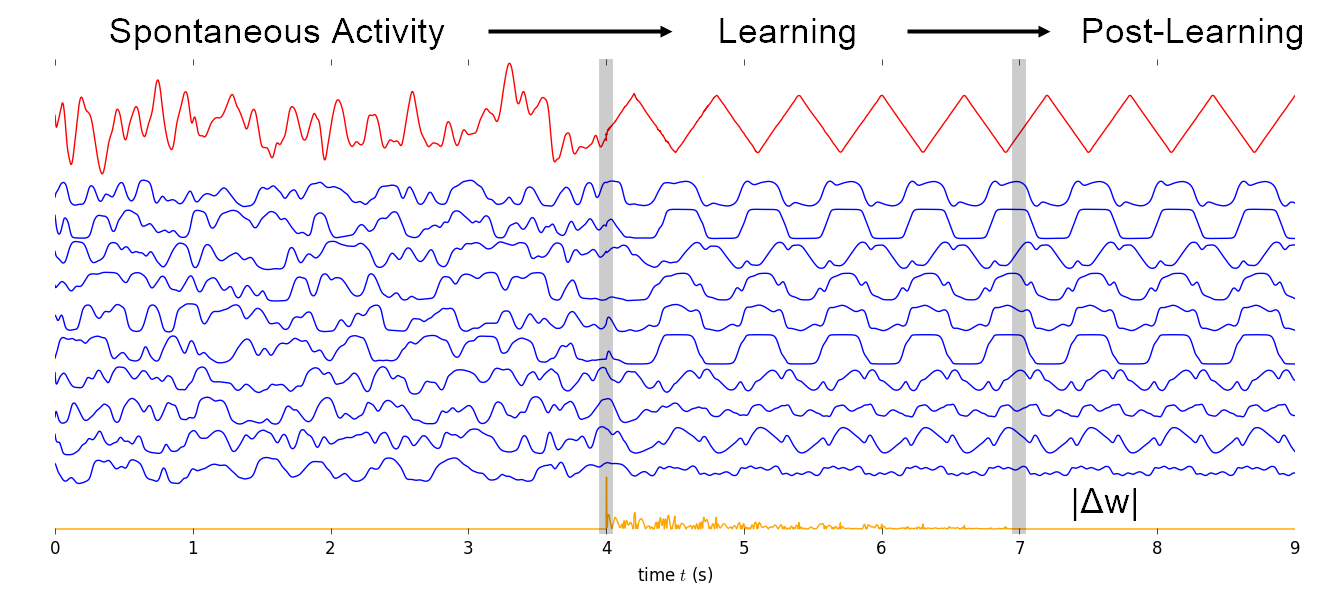
\includegraphics[width=\textwidth]{triangle_text}
  \caption{
    \textbf{FORCE Learning Applied to a Triangle Wave.}\\[0.1 em]
    Network output $z$ is in red, the firing rates of 10 sample neurons
    are in blue and the orange trace represents the magnitude of
    fluctuations of $\mathbf{w}$ 
    ($\Delta \mathbf{w} = \mathbf{w}(t) = \mathbf{w}(t - \Delta t)$).\\[0.1em]
    (A) The network exhibits chaotic spontaneous activity before training.
    \\[0.1em]
    (B) During training, the readout error is reduced to small magnitude 
    rapidly and then the output matches always the target function.
    Readout weights fluctuate greatly at first, gradually the fluctuations
    diminish and finally almost no more modifications of $\mathbf{w}$ are 
    needed.\\[0.1 em]
    (C) At this moment we can turn off the learning procedure and the network 
    persists in generating the desired triangle wave indefinitely
    without requiring any weight modifcation.
  }
  \label{fig: triangle}
\end{figure}

\vfill

\begin{figure}[H]
  \centering
  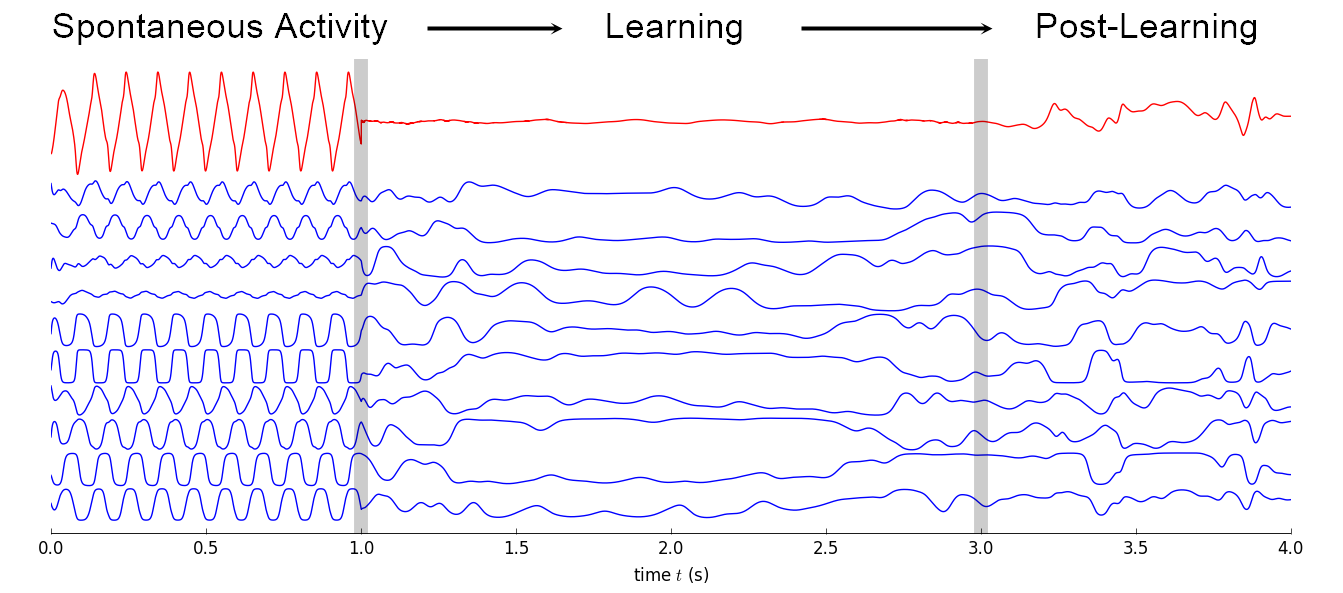
\includegraphics[width=\textwidth]{small_sin_text}
  \caption{
    \textbf{FORCE Learning Applied to Sine wave with Small Magnitude.}
    \\[0.1em]
    FORCE Learning fails for this low amplitude sine wave because
    feedback is not strong enough. What is interesting is that the network
    activity isn't chaotic before training 
    (see text and \autoref{fig: no_chaos})
    but it becomes chaotic during training and remains chaotic after training.
  }
  \label{fig: small_sin}
\end{figure}
\vfill

\newpage

\begin{figure}[H]
  \centering
  \begin{minipage}{0.66\textwidth}
  \begin{subfigure}{0.5\textwidth}
    \centering
    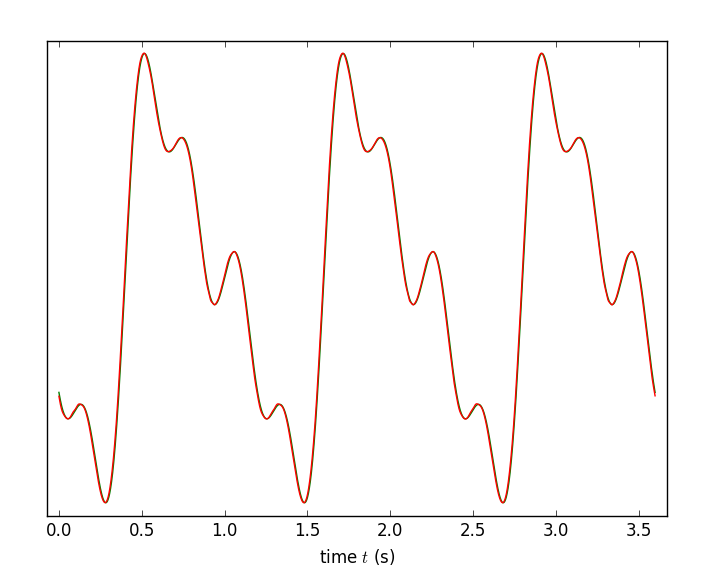
\includegraphics[width=\textwidth]{four_sins}
    \subcaption{Periodic}
  \end{subfigure}
  %
  \begin{subfigure}{0.5\textwidth}
    \centering
    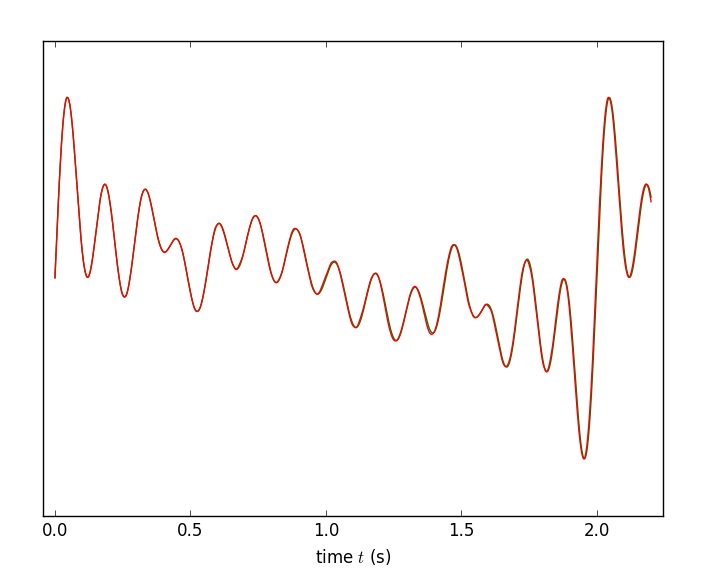
\includegraphics[width=\textwidth]{sixteen_sins}
    \subcaption{Compicated periodic}
  \end{subfigure}
  %
  \begin{subfigure}{0.5\textwidth}
    \centering
    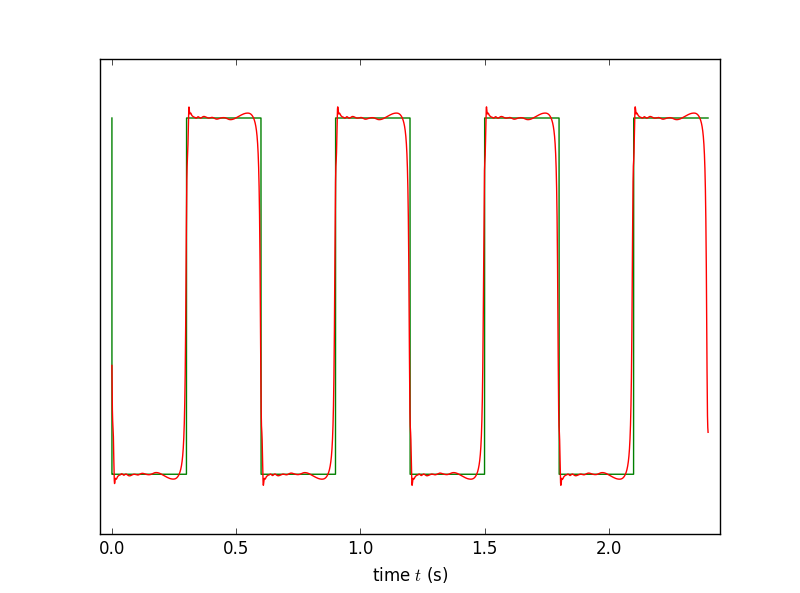
\includegraphics[width=\textwidth]{rectangles}
    \subcaption{Discontinuos target}
  \end{subfigure}
  %
  \begin{subfigure}{0.5\textwidth}
    \centering
    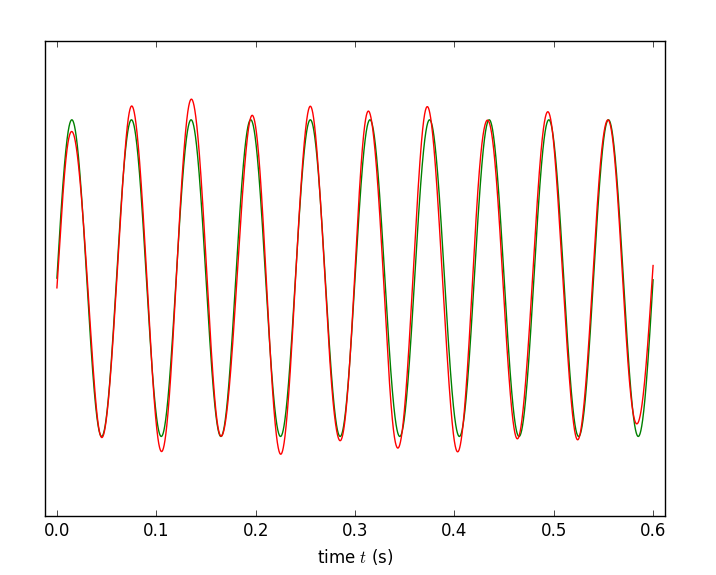
\includegraphics[width=\textwidth]{sin_6tau}
    \subcaption{Sine wave period 6$\tau$}
  \end{subfigure}
  \end{minipage}
  %
  \begin{subfigure}{0.32\textwidth}
    \centering
    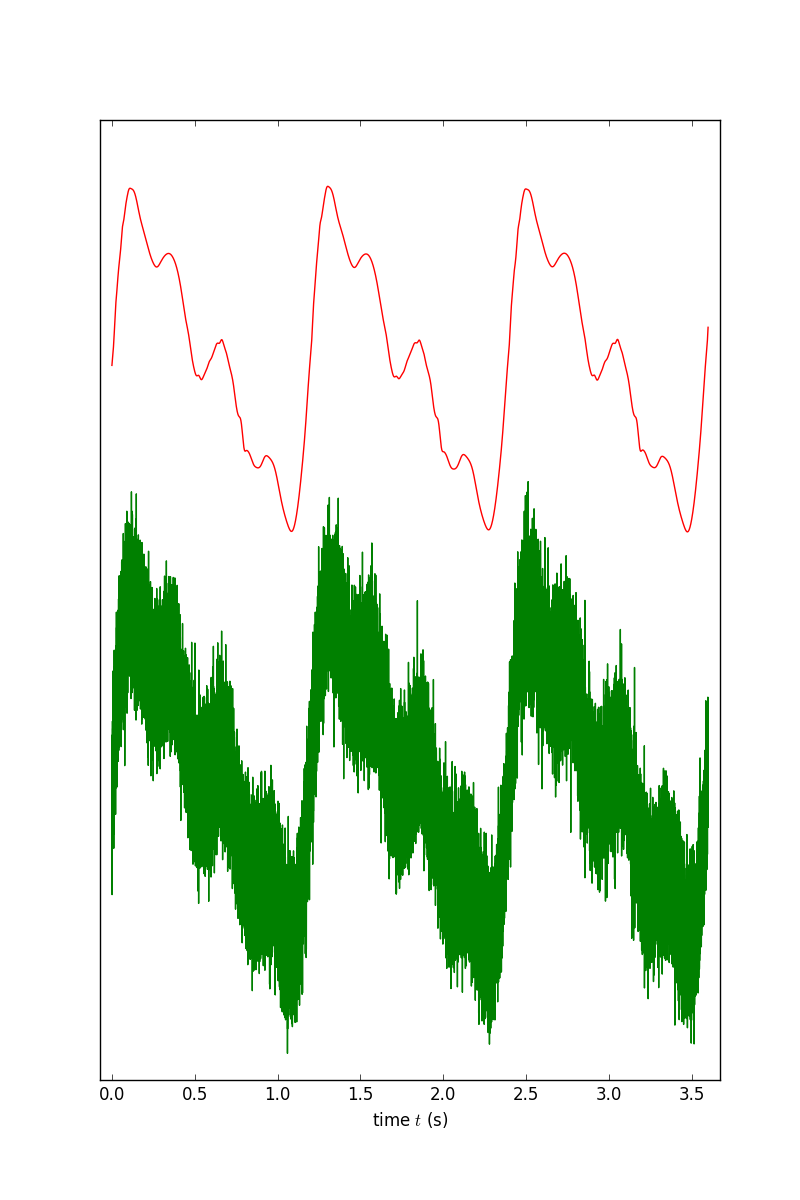
\includegraphics[width=\textwidth]{noisy_four_sins}
    \subcaption{Extremely noisy target}
  \end{subfigure}
  %
  \caption{
    \textbf{FORCE Learning Applied to Various Patterns.}\\[0.1em]
    We show here several examples of successful FORCE learning. 
    Network outputs after training are
    in red and green traces are target functions (often covered by
    the red traces, in subfigure (E) the two traces are separated 
    for a better visualization).\\[0.1em]
    (A) Simple periodic function composed of four sinusoids.\\[0.1em]
    (B) Periodic function composed of sixteen sinusoids.\\[0.1em]
    (C) Square-wave.\\[0.1em]
    (D) Sine wave with pariod of 60 ms.\\[0.1em]
    (E) Periodic function of four sinusoids learned from a noisy target
    functions.
  }
  \label{fig: patterns}
\end{figure}

\vfill

\begin{figure}[H]
  \centering
  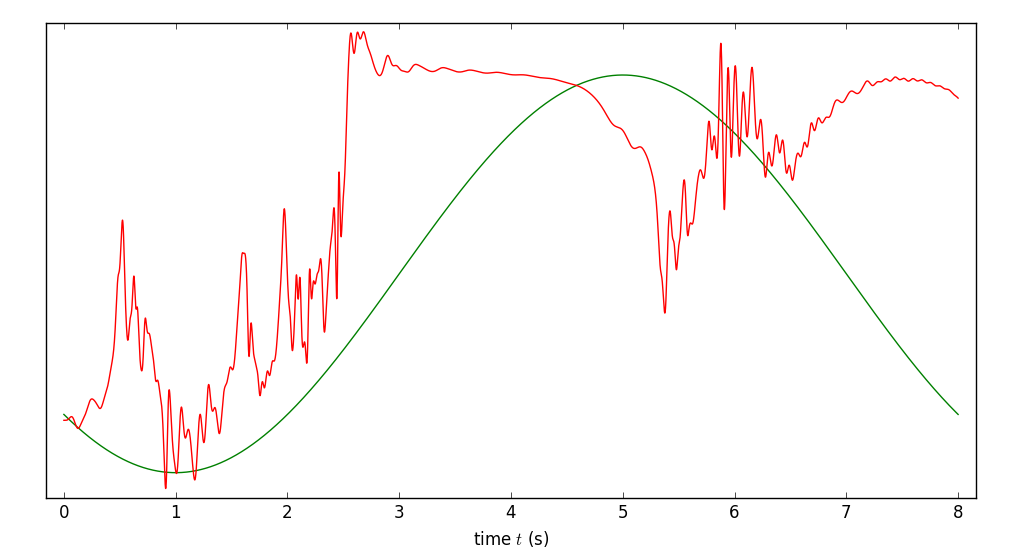
\includegraphics[width=0.7\textwidth]{sin_800tau}
  \caption{
    \textbf{FORCE Learning Applied to a Sine Wave with Period of 8 s.}
    \\[0.1em]
    After one and half of minute of training, the network still
    fails to produce the desired pattern and the generated trace (red)
    doesn't resemble at all the target function (green).
    Either more time is needed for training to converge or this is simply
    an impossible task for the network.
  }
  \label{fig: sin_8s}
\end{figure}
\vfill


\section{Principal Component Analysis of FORCE Learning}

We examine the activity of a network after training by the FORCE procedure
by the usage of principal component analysis (PCA). The network is first
trained to produce the periodic pattern shown in \autoref{fig: PCA}A
(the same target function as \autoref{fig: patterns}A). The distribution
of PCA eigenvalues (\autoref{fig: PCA}C) shows that the trajectory of 
the network activity concentrates on a subspace of much lower dimension
than the number of available neurons in the network. For example, by
projecting the neural activity on the eight leading PC vectors we can
already construct a very good approximation of the real output 
(\autoref{fig: PCA}A).

In the paper, it is shown that after each training, if the readout vector
is projected onto the PC vectors of the network activity, about the top 50 of
these projections converge always to the same specific values. 
In addition, in the RLS algorithm, the matrix $\mathbf{P}$
is adjusted to adapt the learning rates for different PC vectors. 
Nevertheless, further discussion will be omitted here.

\begin{figure}[H]
  \centering
  \begin{subfigure}{0.48\textwidth}
    \centering
    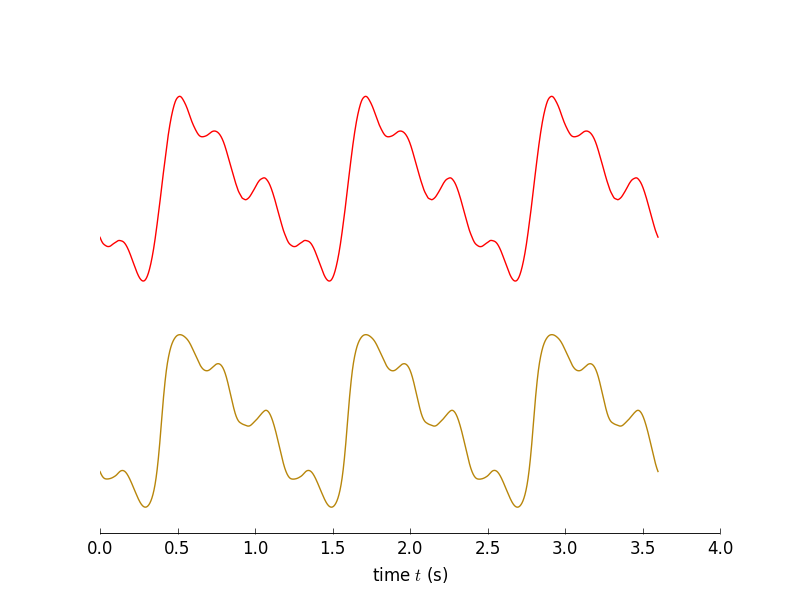
\includegraphics[width=\textwidth]{four_sins_zs_pca}
    \subcaption{}
  \end{subfigure}
  %
  \begin{subfigure}{0.48\textwidth}
    \centering
    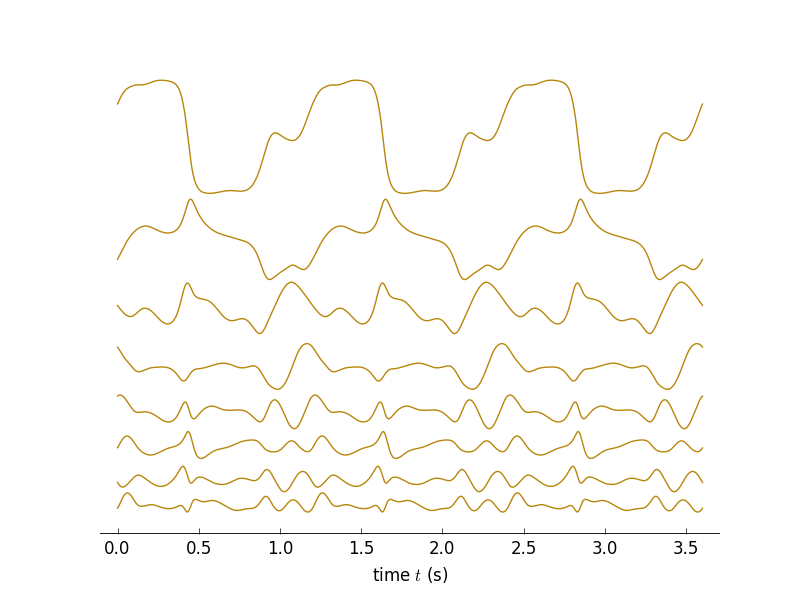
\includegraphics[width=\textwidth]{four_sins_pca8}
    \subcaption{}
  \end{subfigure}
  %
  \flushleft
  \vspace{-1em}
  \hspace{1em}
  \begin{subfigure}{0.6\textwidth}
    \centering
    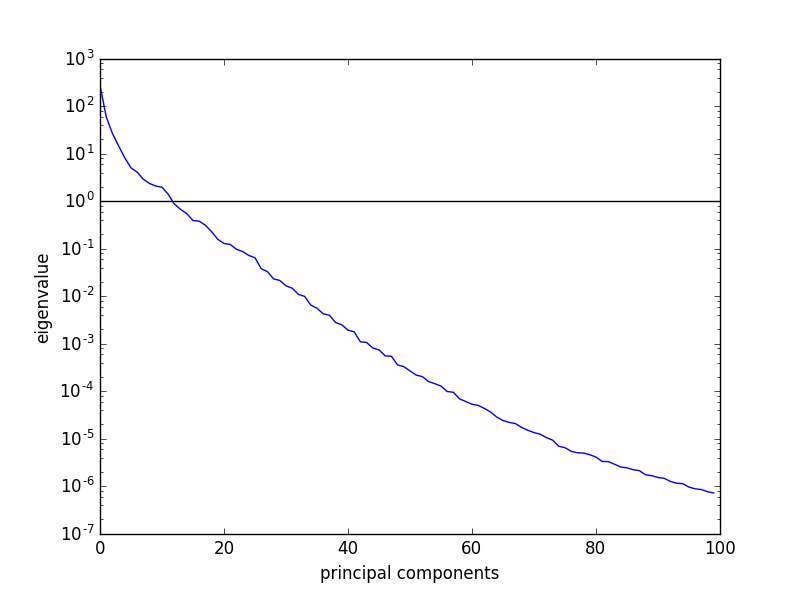
\includegraphics[width=\textwidth]{four_sins_eigenvalues}
    \subcaption{}
  \end{subfigure}
  %
  \caption{
    \textbf{Principal Component Analysis of Netwrok Activity}\\[0.1em]
    (A) Output after training a network to produce a sum of four sinusoids
    (red) and the approximation (brown) obtained using activity
    projected onto the 8 leading principal components.\\[0.1em]
    (B) Projections of network activity onto the leadaing 8 PC vectors.
    \\[0.1em]
    (C) PCA eigenvalues for the network activity. Only the largest 100
    of 1000 eigenvalues are shown.
  }
  \label{fig: PCA}
\end{figure}


\section{Conclusion}

Neural networks in biological systems seem to exhibit complex and
irregular spontaneous activity that has both stochastic and chaotic sources.
In the article ``Generating Coherent Patterns of Activity from
Chaotic Neural Networks'', D. Sussillo and L.F. Abbott propose an 
algorithm called FORCE learning that can endow such
a chaotic network with ability to generate coherent patterns that
may be useful for, for example, motor controls.

In this report I implemented this algorithm on one of the three
network structures given in the article. The network has an linear readout
unit and feedback to the generator network comes directly from this
readout unit. Only readout weights $\mathbf{w}$ are modified during learning.
I was able to reproduce several results shown in the article. After
learning the network manages to generate a variety of periodic
output patterns in the abscence of input, even though all the patterns
presented in the article were not successfully learned 
(sine wave with period 8 s) and the learning time is longer than what
is given in the article. Notice that on a laptop one second in the 
simulation can be much longer in reality, so if the training is meant
to be quite long in simulation the result may not be easily reproducible.
This is in fact the case for Figure 5 in the original text: it's shown
that the performance of the network is the best when it's at the
edge of chaos by training networks of differents values of $g_{GG}$.
It's theoretically easy to reproduce this result because the algorithm
used is exactly as what was implemented in this report. Nevertheless,
too many simulations that are possibly very long are needed to be
carried out to produce a similar figure.

I had also a doubt on the source of the chaotic activity in the model,
since it's not clear if the feedback is connected to the network 
when we say that the network is chaotic before training. PCA carried out on 
the network activity after applying the FORCE procedure is in fact important
to explain how the algorithm works and the final dynamic of the system,
but details are not presented in my report. The paper went much farther
than what has been done until here. The feedback can be distorted and
delayed during training. FORCE algorithm was also adapted
to be used on the network architectures of \autoref{fig: network_structures}B
and 1C. The network can have multiple and multidimensional outputs 
controlable by some particular input signal. Finally, in the paper they
also succeeded in creating a network that can generate multiple,
high-dimensional and nonperiodic patterns that resemble complex human motions.

The FORCE algorithm given here may not be very biologically plausible
(even when applying on the second and the third network structure)
because updates of readout weights rely on a global error and another
global quantity $\mathbf{P}$. A simpler plasticity mechanism is proposed 
by D. Sussillo and L.F. Abbott in the supplemental data of their article,
but on the other hand it's not as powerful as the version presented here.

Another surprising fact is that through out the report, at no time we're
modifying the internal recurrent synaptic strengths of the network, but
the network is still able to produced the desired patterns after training.
Only looking at the internal synaptic connectivity, we would not be able
to tell what the network is doing. Feedback loops passing through distal
networks may play a role far more important than one imagines. This
also means that the network is able to learn new tasks without need to
have great modifications on the orignial circuit whose synaptic
connectivity are probably already fixed from some more basic tasks to
be carried out.
